\chapter{CONCEITOS FUNDAMENTAIS}\label{chap:conceitos}

Este capítulo apresenta as métricas que serão utilizadas no classificador e realiza uma breve introdução aos conceitos de mecânica quântica necessários para compreender a estrutura de um computador quântico e como eles podem ser empregados para tarefas de \textit{machine learning}.

\section{Métricas de Avaliação}

As métricas de avaliação desempenham um papel de extrema importância em projetos que envolvem aprendizado de máquina, uma vez que permitem uma avaliação numérica do progresso alcançado. As tarefas de aprendizado de máquina podem ser classificadas em regressão ou classificação, assim como as métricas utilizadas para avaliação. Embora existam várias métricas para ambas as áreas, esta seção se concentrará nas métricas de avaliação mais populares para classificação, tais como \textit{recall}, especificidade, acurácia, precisão, \textit{F1-score} e AUC-ROC.

Conforme mencionado por \citeonline{Métricas}, no contexto da classificação binária, ou seja, problemas em que cada amostra pertence a uma de duas classes, convencionalmente denominadas positiva e negativa, as predições podem ser classificadas da seguinte forma:

\begin{itemize}
\item \textbf{Verdadeiro positivo (VP)}: o modelo realizou a predição de que a classe é positiva e realmente é positiva;
\item \textbf{Verdadeiro negativo (VN)}: o modelo realizou a predição de que a classe é negativa e realmente é negativa;
\item \textbf{Falso positivo (FP)}: o modelo realizou a predição de que a classe é positiva, porém ela é negativa;
\item \textbf{Falso negativo (FN)}: o modelo realizou a predição de que a classe é negativa, porém ela é positiva;
\end{itemize}

\subsection{Matriz de Confusão}

\begin{figure}[H]
\begin{center}
\caption{Matriz de Confusão.}
\begin{tikzpicture}[
box/.style={draw,rectangle,minimum size=2cm,text width=2cm,align=left}]
\matrix (conmat) [row sep=.1cm,column sep=.1cm] {
\node (tpos) [box,
    label=left:\( \mathbf{p'} \),
    label=above:\( \mathbf{p} \),
    ] {Verdadeiro \\ positivo};
&
\node (fneg) [box,
    label=above:\textbf{n},
    label=above right:\textbf{total},
    label=right:\( \mathrm{P}' \)] {Falso \\ negativo};
\\
\node (fpos) [box,
    label=left:\( \mathbf{n'} \),
    label=below left:\textbf{total},
    label=below:P] {Falso \\ positivo};
&
\node (tneg) [box,
    label=right:\( \mathrm{N}' \),
    label=below:N] {Verdadeiro \\ negativo};
\\
};
\node [left=.05cm of conmat,text width=1.5cm,align=right] {\textbf{Valor \\ atual}};
\node [above=.05cm of conmat] {\textbf{Resultado Previsto}};
\end{tikzpicture}
\smallcaption{Fonte: Autor.}
\end{center}
\end{figure}

A matriz de confusão resume o número de instâncias nas categorias VP, VN, FP e FN, descrevendo o desempenho do modelo. Cada linha da matriz representa as instâncias em uma classe prevista, e cada coluna representa as instâncias em uma classe real. A matriz de confusão não é exatamente uma métrica, mas uma espécie de base na qual os resultados das métricas são avaliados.

\subsection{Recall}

O \textit{recall} ou sensibilidade é a fração de amostras de uma classe que são previstas corretamente pelo modelo. É calculado como a razão entre os verdadeiros positivos e a soma de verdadeiros positivos e falsos negativos \cite{Métricas}:

\begin{center}
\begin{equation}
\text{Recall} = \dfrac{\text{VP
}}{\text{VP} + \text{FN}}
\end{equation}
\end{center}

\subsection{Especificidade}

A especificidade avalia a capacidade do método de encontrar resultados negativos. É calculada utilizando a fórmula \cite{Métricas}:

\begin{center}
\begin{equation}
\text{Especificidade} = \dfrac{\text{VN}}{\text{VN} + \text{FP}}
\end{equation}
\end{center}

\subsection{Acurácia}

A acurácia é talvez a métrica mais simples de ser implementada e é definida como o número de previsões corretas dividido pelo número total de previsões.

Utilizando a matriz de confusão como base, podemos obter a acurácia do modelo utilizando a fórmula \cite{Métricas}:

\begin{center}
\begin{equation}
\text{Acurácia} = \dfrac{\text{VP} + \text{VN}}{\text{VP} + \text{FP} + \text{FN} + \text{VN}}
\end{equation}
\end{center}

\subsection{Precisão}

A precisão é a razão entre os verdadeiros positivos e o total de positivos previstos. Podemos obtê-la por meio da fórmula \cite{Métricas}:

\begin{center}
\begin{equation}
\text{Precisão} = \dfrac{\text{VP}}{\text{VP} + \text{FP}}
\end{equation}
\end{center}

\subsection{F1-score}

O \textit{F1-score} utiliza uma combinação de precisão e \textit{recall}. É calculado como a média harmônica entre essas duas métricas. A fórmula é \cite{Métricas}:

\begin{center}
\begin{equation}
\text{F1-score} = 2 \times \dfrac{\text{Precisão} \times \text{Recall}}{\text{Precisão} + \text{Recall}}
\end{equation}
\end{center}


\subsection{AUC-ROC}

A "área sob a curva" (AUC) refere-se à área sob a curva ROC. Essa área captura a capacidade do modelo de distinguir entre as classes positivas e negativas, independentemente do ponto de corte escolhido. Um modelo perfeito terá uma AUC de 1, enquanto um modelo aleatório (sem poder discriminativo) terá uma AUC de 0.5.

Para calcular a AUC-ROC, é comum utilizar a regra do trapézio para aproximar a área sob a curva ROC. Para um modelo de classificação binária, a fórmula para calcular a AUC-ROC é \cite{Métricas}:

\begin{center}
\begin{equation}
\text{AUC ROC} = \int_{0}^{1} \text{Recall}(1-\text{Especificidade}) , d(1-\text{Especificidade})
\end{equation}
\end{center}

Com essas métricas, é possível avaliar de maneira eficiente o desempenho de um modelo de classificação. Cada métrica possui sua importância e pode ser mais adequada para um determinado tipo de problema ou conjunto de dados. Portanto, é fundamental compreender as características e necessidades do problema em questão a fim de selecionar as métricas mais apropriadas para avaliar o desempenho do modelo.


\section{Computação Quântica}

%\chapter{CONCEITOS FUNDAMENTAIS}\label{chap:conceitos}

Nas primeiras décadas do século passado, houve uma transformação drástica na compreensão do mundo. A visão determinística clássica da mecânica e eletrodinâmica, que buscava descrever todos os fenômenos físicos, revelou-se insuficiente diante de certos experimentos. A hipótese quântica surgiu inicialmente com Max Planck, que buscou descrever o fenômeno da radiação térmica, e posteriormente foi desenvolvida por Schrödinger, Dirac \cite{Dirac} e outros físicos.

A mecânica quântica difere das teorias clássicas, e o Princípio da Incerteza de Heisenberg \cite{Mermin2007QComputerScience} ilustra essa diferença ao afirmar que a medição do estado de um sistema afeta o próprio estado do sistema em questão. No caso de uma partícula, isso significa que não é possível medir simultaneamente e com precisão arbitrária a posição $x$ e a componente $p_x=mv_x$ do momento linear, onde $m$ é a massa e $v_x$ é a componente da velocidade da partícula. Em vez disso, as incertezas $\Delta x$ e $\Delta p$ devem obedecer à desigualdade
\begin{equation} \label{eq:incerteza}
\Delta x \Delta p \geq \frac{\hbar}{2}
\end{equation}
\noindent onde $\hbar=h/2\pi$ é a constante de Planck dividida por $2\pi$.

Na mecânica quântica, as grandezas físicas, como $x$ e $p_x$, são representadas por operadores lineares $\hat{x}$ e $\hat{p}_x$, e os resultados das medições correspondem aos autovalores desses operadores \cite{Zubairy2020}. Os operadores lineares podem ser representados por matrizes, e essas matrizes podem não comutar, o que implica que elas não possuem autovetores comuns. Nesse caso, a medição de uma grandeza física afeta a medição da outra grandeza. A equação \ref{eq:incerteza} é consequência da relação de comutação
\begin{equation} \label{eq:heisenberg}
\hat{x}\hat{p}_x - \hat{p}_x \hat{x} = i\hbar
\end{equation}
\noindent entre as matrizes que representam as grandezas físicas posição e momento linear \cite{Zubairy2020}.

Em 1981, Richard Feynman e Yuri Manin propuseram os computadores quânticos \cite{Wong2022IntroductionClassicalQuantum}, e em 1985, David Deutsch descreveu matematicamente o primeiro computador quântico equivalente a uma máquina de Turing quântica \cite{Mermin2007QComputerScience}. Desde então, algoritmos e computadores quânticos foram desenvolvidos. Em resumo, um computador quântico é uma máquina cujo processamento é baseado nas propriedades quânticas da natureza. Nos próximos capítulos, serão abordados os conceitos necessários para compreender o funcionamento dos computadores quânticos, bem como os algoritmos de \textit{quantum machine learning}.

\subsection{Formalismo matemático} \label{formalismo}

Para compreendermos os conceitos que permeiam a computação quântica, faremos uso do simbolismo introduzido por Dirac \cite{Dirac}. Essa notação foi criada para expressar estados, produtos internos e operadores na mecânica quântica. O estado de um sistema é descrito por um vetor $\ket{\psi}$, conhecido como ket, e representado por uma matriz coluna, ou por um vetor $\bra{\psi}$, denominado bra, e representado por uma matriz linha. O produto interno entre dois vetores é um número complexo e é denotado por um bra-ket $\braket{\phi | \psi}$. Os operadores são matrizes quadradas construídas a partir de operadores de projeção, como $\ket{\psi}\bra{\phi}$ \cite{Dirac,Mermin2007QComputerScience,Zubairy2020,Wong2022IntroductionClassicalQuantum}.

\subsection{Bits e Qubits} \label{Qubits}

O qubit é o análogo quântico do bit clássico. Na computação clássica, o bit pode representar dois valores, 0 ou 1. Por outro lado, o qubit é um sistema quântico que possui dois estados básicos representados pelos vetores $\ket{0}$ e $\ket{1}$, denominados estados da base computacional \cite{Nielsen,Mermin2007QComputerScience}.

Diferentemente dos bits clássicos, os qubits podem estar em um estado de superposição, que consiste em uma combinação linear dos dois estados da base computacional:
%
%
\begin{center}
\begin{equation}
\ket{\psi} = \alpha_0\ket{0} + \alpha_1\ket{1} 
\end{equation}
\end{center}
%
%
\noindent sendo que os coeficientes $\alpha_0$ e $\alpha_1$ são números complexos chamados amplitudes por analogia com a superposição de ondas. A regra de Born permite associar as amplitudes com probabilidades \cite{Dirac,Nielsen,Mermin2007QComputerScience,Zubairy2020,Wong2022IntroductionClassicalQuantum}: quando um qubit está no estado descrito por $\ket{\psi}$, a probabilidade de que o resultado de uma medição na base computacional corresponda ao estado $\ket{0}$ é $P(0)=|\alpha_0|^2$ enquanto a probabilidade de o resultado da medição corresponder ao estado $\ket{1}$ é $P(1)=|\alpha_1|^2$. Como as amplitudes $\alpha_0$ e $\alpha_1$ levam à determinação de probabilidades, é necessário que sejam normalizadas, isto é, 
%
%
\begin{center}
\begin{equation}
 |\alpha_0|^2 + |\alpha_1|^2 = 1 
\end{equation}
\end{center}
%
%
\noindent a fim de garantir a interpretação probabilística adequada.

Aqui, é importante ressaltar que a superposição é uma propriedade única dos sistemas quânticos e permite que um qubit possa existir em um estado que é uma combinação dos estados básicos $\ket{0}$ e $\ket{1}$ \cite{Wong2022IntroductionClassicalQuantum}. Essa superposição permite que os computadores quânticos processem informações de maneira paralela, o que pode lhes conferir uma vantagem potencial de processamento em comparação aos computadores clássicos.

Na representação geométrica, um qubit pode ser visualizado na Esfera de Bloch \cite{Wong2022IntroductionClassicalQuantum}, onde os estados puros $\ket{0}$ e $\ket{1}$ estão localizados nos polos norte e sul, respectivamente. Estados de superposição são representados por pontos na superfície da esfera e o vetor de estado quântico, também conhecido como vetor de Bloch, aponta para o estado atual do qubit.

\begin{figure}[H]
\centering
\caption{Esfera de Bloch.}
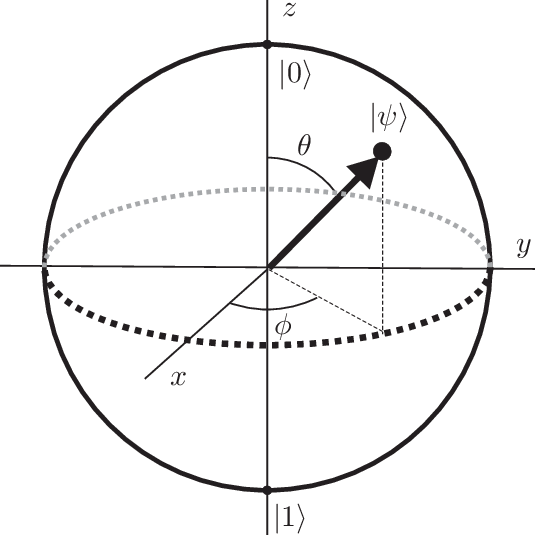
\includegraphics[scale=0.3]{imagens/bloch_sphere.png}
\smallcaption{Fonte: Wikipedia.}
\label{fig:figura_3}
\end{figure}

A representação física de um qubit pode ser a polarização de um fóton, o estado de \textit{spin} de uma partícula, dois níveis de energia de um átomo ou de um transmon, entre outros. Computadores clássicos realizam cálculos baseando-se em \textit{strings} de bits, como por exemplo 01010. Por outro lado, computadores quânticos assimilam múltiplos qubits usando produto tensorial, portanto essa mesma sequência pode ser escrita como:

\begin{center}
\begin{equation}
\ket{\psi} = \ket{0} \otimes \ket{1} \otimes \ket{0} \otimes \ket{1} \otimes \ket{0} = | 01010 \rangle
\end{equation}
\end{center}

É importante ressaltar que em uma superposição geral de 5 qubits teríamos:

\begin{center}
\begin{equation}
\ket{\psi} = \alpha_1\ket{00000} + \alpha_2\ket{00001} + \ldots + \alpha_{32}\ket{11111}
\end{equation}
\end{center}

\noindent onde $\alpha_i \in \mathbb{C}$ são coeficientes complexos que obedecem à relação de normalização $\sum_{i=1}^{32}|\alpha_i|^2 = 1$ \cite{Wong2022IntroductionClassicalQuantum}.

O emaranhamento é outra característica única da mecânica quântica que pode ser usada como recurso na computação quântica. Para compreender o emaranhamento, precisamos introduzir a noção de estados separáveis. No caso de dois qubits, uma superposição 

\begin{center}
\begin{equation}
\ket{\psi} = \alpha_{00}\ket{00} + \alpha_{01}\ket{01} +\alpha_{10}\ket{10} + \alpha_{11}\ket{11}   
\end{equation}
\end{center}

\noindent é separável se puder ser escrita como o produto tensorial $\ket{\psi_1}\otimes\ket{\psi_2}$ dos estados $\ket{\psi_1}$ e $\ket{psi_2}$, cada um dos quais pertencentes a um subespaço vetorial \cite{Wong2022IntroductionClassicalQuantum}. Assim, o estado é separável porque pode ser escrito como: 

\begin{center}
\begin{equation}
\ket{\psi} = \frac{1}{2}(\ket{00} + \ket{01} - \ket{10} - \ket{11})   
\end{equation}
\end{center}

\begin{center}
\begin{equation}
\ket{\psi} = \left(\frac{1}{\sqrt{2}}(\ket{0} - \ket{1}\right)\otimes\left(\frac{1}{\sqrt{2}}(\ket{0} + \ket{1}\right).   
\end{equation}
\end{center}

Uma característica de um estado separável como $\ket{\psi}$ é que saber o resultado de uma medição realizada sobre um dos qubits não fornece informação sobre o resultado de uma medição feita sobre o outro qubit. Em um estado separável, os qubits se comportam como se fossem independentes uns dos outros.  

Por outro lado, um estado de Bell como:

\begin{center} \label{eq:Bell}
\begin{equation}
\ket{\Psi^-} = \frac{1}{\sqrt{2}}(\ket{01} - \ket{10}). 
\end{equation}
\end{center}

Não é separável e é chamado emaranhado \cite{Wong2022IntroductionClassicalQuantum}. A característica especial de um estado emaranhado é que os resultados das medições sobre um dos qubits estão fortemente correlacionadas com os resultados das medições sobre o outro qubit. No caso do estado $\ket{\Psi^-}$, saber o resultado de uma medição realizada sobre um dos qubits permite prever com certeza absoluta o resultado de uma medição feita sobre o outro qubit, mesmo que os dois qubits estejam muito distantes quando forem medidos. Neste caso, os qubits não são independentes uns dos outros.  


\subsection{Portas Lógicas Quânticas} \label{Portas}

O processamento de informação exige que o computador seja capaz de alterar o estado dos qubits que armazenam informação. No modelo de circuito da computação quântica, a modificação do estado dos qubits é representada pela aplicação de uma sequência de portas lógicas quânticas aos qubits do computador quântico \cite{Nielsen}. Portas quânticas são operadores lineares que realizam transformações unitárias em qubits, preservando a normalização dos estados. Como a ação de um operador linear $U$ sobre uma superposição é

\begin{center}
\begin{equation}
  U(\alpha_0\ket{0} + \alpha_1\ket{1}) = \alpha_0 U\ket{0} +\alpha_1 U\ket{1},
\end{equation}
\end{center}

\noindent então uma porta quântica pode ser caracterizada por sua ação sobre os vetores da base computacional. 

A porta quântica $X$, por exemplo, é caracterizada por:

\begin{center}
\begin{equation}
\begin{aligned}
X\ket{0} &= \ket{1}, \\
X\ket{1} &= \ket{0}.
\end{aligned}
\end{equation}
\end{center}

\noindent correspondendo a uma generalização quântica da porta lógica clássica NOT. Em termos geométricos, a porta $X$ corresponde a uma rotação de $\pi$ do vetor de estado em torno do eixo $x$ da esfera de Bloch:

\begin{center}
\begin{equation}
X (\alpha_0\ket{0} + \alpha_1\ket{1}) = \alpha_1 \ket{0} + \alpha_0 \ket{1},
\end{equation}
\end{center}

\noindent que corresponde a trocar as amplitudes e, portanto, as probabilidades associadas a cada estado da base computacional. Assim como os qubits, é possível representar as portas quânticas em forma matricial, como podemos ver com a porta $X$:

\begin{center}
\begin{equation}
X =
\begin{pmatrix}
0 & 1\\
1 & 0
\end{pmatrix}
\end{equation}
\end{center}

Ao contrário da computação clássica que possui poucas portas lógicas de um bit, a computação quântica admite infinitas portas quântica de um qubit \cite{Nielsen}. Abaixo, podemos observar algumas portas lógicas quânticas de um qubit e suas respectivas representações matriciais e de Dirac:

\begin{figure}[H]
    \centering
    \caption{Portas lógicas quânticas de um qubit.}
    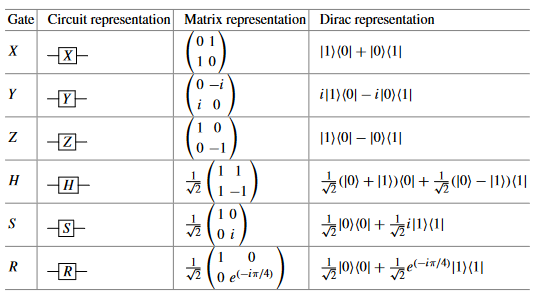
\includegraphics[scale=0.75]{imagens/Tabela_Portas.png}
    \smallcaption{Fonte: \cite{Schuld2021MLQComputers}}
    \label{fig:portas_quanticas}
\end{figure}

A porta $Z$ é especial porque os estados $\ket{0}$ e $\ket{1}$ da base computacional são os seus dois autoestados. A porta $Z$ realiza uma rotação de $\pi$ em torno do eixo $z$ da esfera de Bloch, invertendo o sinal do estado $\ket{1}$ \cite{Nielsen}:

\begin{center}
\begin{equation}
Z (\alpha_0\ket{0} + \alpha_1\ket{1}) = \alpha_0 \ket{0} - \alpha_1 \ket{1} = \alpha_0 \ket{0} + e^{i\pi}\alpha_1 \ket{1}).
\end{equation}
\end{center}
\noindent A inversão de sinal do estado $\ket{1}$ corresponde à introdução de uma fase relativa $\pi$ entre os dois estados $\ket{0}$ e $\ket{1}$ na superposição. 

A porta $Y$, por sua vez, realiza uma rotação de $\pi$ em torno do eixo $y$ da esfera de Bloch, mudando o estado do qubit da seguinte maneira \cite{Nielsen}:

\begin{center}
\begin{equation}
Y (\alpha_0\ket{0} + \alpha_1\ket{1}) = -i\alpha_1 \ket{0} + i\alpha_0 \ket{1} = e^{-i\pi/2}(\alpha_1 \ket{0} + e^{i\pi}\alpha_0 \ket{1})
\end{equation}
\end{center}
\noindent que é uma espécie de combinação dos efeitos das portas $X$ e $Z$ ao trocar as amplitudes e introduzir uma fase relativa entre as componentes $\ket{0}$ e $\ket{1}$ da superposição. 

As portas $X$, $Y$ e $Z$ são chamadas portas de Pauli porque são equivalentes às matrizes de Pauli utilizadas para representação de partículas de spin $1/2$ como elétrons, prótons ou nêutrons. Além das portas de Pauli, existem as portas de fase como as portas $S$ e $R$. A porta $S$ introduz uma fase relativa $\pi/2$ no estado $\ket{1}$, realizando uma rotação de $\pi/2$ em torno do eixo $z$ na esfera de Bloch, levando o estado $\ket{0}$ no próprio estado $\ket{0}$ e o estado $\ket{1}$ no estado $i\ket{1}$ \cite{Nielsen}.

Por fim, temos a porta $R$, que é uma porta de fase geral representada por uma matriz diagonal com um parâmetro $\phi$. Ela adiciona uma fase $e^{i\phi}$ ao estado $\ket{1}$. A porta $R$ também realiza uma rotação em torno do eixo $z$ na esfera de Bloch, dependendo do valor do ângulo $\phi$ \cite{Nielsen}.

Além das portas de Pauli e das portas de fase, existem as portas de rotação, que serão importantes no desenvolvimento deste trabalho. A porta $R_x(\theta)$ é dada, em forma matricial por

\begin{center}
\begin{equation}
R_x(\theta) =
\begin{pmatrix}
\cos(\theta/2) & -i\sin(\theta/2) \\
-i\sin(\theta/2) & \cos(\theta/2)
\end{pmatrix}
\end{equation}
\end{center}

\noindent e representa uma rotação por um ângulo $\theta$ em torno do eixo $x$ da esfera de Bloch. De maneira semelhante, a porta $R_y(\theta)$, que representa uma rotação por um ângulo $\theta$ em torno do eixo $y$ da esfera de Bloch é dada por

\begin{center}
\begin{equation}
R_y(\theta) =
\begin{pmatrix}
\cos(\theta/2) & -\sin(\theta/2) \\
\sin(\theta/2) & \cos(\theta/2)
\end{pmatrix}
\end{equation}
\end{center}

\noindent e a porta $R_z(\theta)$ é 

\begin{center}
\begin{equation}
R_z(\theta) =
\begin{pmatrix}
e^{-i\theta/2} & 0            \\
0              & e^{i\theta/2}
\end{pmatrix}
\end{equation}
\end{center}

\noindent As portas de Pauli são casos especiais das portas de rotação: $X=iR_x(\pi)$, $Y=iR_y(\pi)$ e $Z=iR_z(\pi)$ \cite{Zubairy2020}.

Provavelmente a porta de um qubit mais notável é a porta $H$ ou porta de Hadamard. Enquanto as portas de Pauli são parecidas com portas lógicas clássicas em alguns aspectos, a porta de Hadamard não se assemelha a nenhuma porta lógica clássica \cite{Mermin2007QComputerScience}. Ela é capaz de transformar um estado quântico como $\ket{0}$ em uma superposição uniforme, fazendo com que a probabilidade da medição de 0 seja igual à probabilidade de medição de 1. Podemos representar esse processo como:

%\begin{equation}
%\begin{centering}
%\begin{quantikz}
%  \lstick{$\ket{1}$} & \gate{H} & \rstick{$\frac{1}{\sqrt{2}}(\ket{0} + \ket{1})$}
%\end{quantikz}
%\end{centering}
%\end{equation}

\begin{equation}
\begin{centering}
\text{H}\ket{0} = \frac{1}{\sqrt{2}}(\ket{0} + \ket{1}).
\end{centering}
\end{equation}

\noindent Aqui, a saída da porta de Hadamard é representada pelo estado $\ket{+} = (\ket{0} + \ket{1})/\sqrt{2}$, que indica uma superposição igualmente provável dos estados $\ket{0}$ e $\ket{1}$. De acordo com a regra de Born \cite{Nielsen}, a probabilidade de medir os estados $\ket{0}$ e $\ket{1}$ é igual, ou seja, $P(0) = P(1) = 1/2$. Aplicando a porta de Hadamard em um qubit com estado $\ket{1}$, temos a seguinte transformação:

\begin{equation}
\begin{centering}
\text{H}\ket{1} = \frac{1}{\sqrt{2}}(\ket{0} - \ket{1}),
\end{centering}
\end{equation}

\noindent que corresponde ao estado $\ket{-} = (\ket{0} - \ket{1})/\sqrt{2}$ que é outra superposição uniforme dos estados $\ket{0}$ e $\ket{1}$. Como $\braket{-}{+} = 0$, os estados $\ket{+}$ e $\ket{-}$ são ortogonais e poderiam ser usados como uma base computacional alternativa \cite{Nielsen}.


Além das portas quânticas de um qubit, existem portas quânticas que operam em mais de um qubit, como a porta $cX$, que é a generalização quântica da porta lógica CNOT (Controlled NOT) e a porta de Toffoli \cite{Nielsen}. A porta $cX$ é uma porta de dois qubits que atua como uma porta NOT no segundo qubit se o primeiro qubit estiver no estado $\ket{1}$. A porta de Toffoli, por sua vez, é uma porta de três qubits que atua como uma porta NOT no terceiro qubit se os dois primeiros qubits estiverem no estado $\ket{11}$.

Essas portas quânticas desempenham um papel fundamental na manipulação e transformação de estados quânticos de um qubit. Elas permitem a realização de operações complexas, como superposição, inversão de fase e rotação nos estados quânticos, abrindo caminho para a construção de algoritmos e protocolos quânticos poderosos. A compreensão das portas quânticas é fundamental para o desenvolvimento e aplicação de algoritmos quânticos em aprendizado de máquina e outras áreas da computação quântica \cite{Biamonte2017QML, Wong2022IntroductionClassicalQuantum}.

\subsection{Medição de Qubits} \label{Medicao}

A medição é um aspecto fundamental da mecânica quântica e desempenha um papel crucial na computação quântica. De acordo com os postulados da mecânica quântica, a medição de um observável $A$, como posição, energia ou momento linear, resultará em um e apenas um dos autovalores de $A$, com a probabilidade determinada pelo estado quântico do sistema antes da medição \cite{Nielsen}.

Ao contrário das portas lógicas quânticas, a medição é uma operação irreversível que causa o colapso do estado quântico. Após a medição, o estado quântico se torna o autovetor correspondente ao autovalor medido, e todas as informações sobre a superposição anterior e as fases relativas são perdidas \cite{Nielsen}.

Para ilustrar o processo de medição, considere o seguinte circuito quântico:

\begin{figure}[H]
\begin{center}
\caption{Exemplo de circuito quântico.}
\begin{quantikz}
\lstick{$\ket{0}$} & \gate{H} & \ctrl{1} & \meter{} & \rstick{$c_0$} \\
\lstick{$\ket{0}$} & \gate{H} & \targ{}  & \meter{} & \rstick{$c_1$}
\end{quantikz}
\end{center}
\smallcaption{Fonte: Autor.}
\label{fig:circ_quant}
\end{figure}

O circuito acima representa um exemplo simples que cria um par emaranhado de qubits. Após a criação do par emaranhado, o circuito mede os qubits e armazena os resultados em bits clássicos. O símbolo \begin{quantikz}& \meter{} \end{quantikz} indica a medição no circuito.

Executando-se o circuito diversas vezes, é possível obter as probabilidades dos estados $\ket{0}$ e $\ket{1}$. Se o estado quântico for uma superposição igual de $\ket{0}$ e $\ket{1}$, a probabilidade de medir cada estado seria de 50\% \cite{Nielsen}. No entanto, devido à presença de ruídos e imperfeições nos dispositivos quânticos atuais, os resultados experimentais podem apresentar desvios em relação às probabilidades teóricas ideais \cite{Wong2022IntroductionClassicalQuantum}.

A medição é um processo fundamental na computação quântica, pois permite extrair informações úteis dos estados quânticos e aplicá-las em algoritmos e aplicações práticas. No entanto, a natureza irreversível da medição também impõe limitações, como a destruição da superposição e do emaranhamento. Por isso, o desenvolvimento de algoritmos quânticos eficientes e a melhoria dos dispositivos quânticos para reduzir o impacto do ruído são desafios importantes na pesquisa em computação quântica \cite{Schuld2021MLQComputers}.

\section{Método de Codificação de Input} \label{Encoding}

A codificação de dados clássicos em computadores quânticos é um problema em aberto e depende do contexto e do problema em estudo \cite{Schuld2021MLQComputers}. Existem várias abordagens para codificar informações clássicas em estados quânticos, como \textit{Basis Encoding}, \textit{Amplitude Encoding}, \textit{Feature Map Encoding}, \textit{Time-Evolution Encoding} e \textit{Hamiltonian Encoding}. Nesta seção, será abordado apenas o método de codificação utilizado no desenvolvimento deste projeto: \textit{Feature Map Encoding}.

\subsection{Feature Map Encoding}

A Codificação de Mapa de Características, também conhecida como \textit{Feature Map Encoding}, é um método de codificação de dados clássicos em estados quânticos, comumente usado em aprendizado de máquina quântico \cite{Havlicek2019qSupervisedLearning}. Nesse método, os dados clássicos são mapeados em um espaço de características quânticas através de uma função não linear. O mapeamento é projetado para preservar e realçar as propriedades relevantes dos dados clássicos para o problema em questão, facilitando o processo de aprendizado.

Um exemplo de mapa de características é a transformada de dados clássicos em ângulos de rotação de portas quânticas de rotação. Considere um vetor de dados clássicos $(x_1, x_2)$. Para mapear esses dados em um espaço de características quânticas, aplicamos portas de rotação nos qubits de acordo com os valores $x_1$ e $x_2$. Por exemplo, podemos aplicar uma porta de rotação $R_x(\theta_1)$ no primeiro qubit usando o ângulo de rotação $\theta_1 = \pi x_1$ e uma porta de rotação $R_y(\theta_2)$ no segundo qubit com o ângulo de rotação $\theta_2 = \pi x_2$. O resultado é um estado quântico que codifica as informações dos dados clássicos de maneira não linear.

A Codificação de Mapa de Características é o método de codificação utilizado no desenvolvimento do classificador deste projeto. Essa abordagem permite explorar as propriedades quânticas, como a superposição e o emaranhamento, e pode resultar em algoritmos de aprendizado de máquina mais eficientes quando comparados aos métodos clássicos. No entanto, é importante observar que a escolha do mapa de características adequado é uma tarefa desafiadora e depende do problema específico em estudo.

\section{Aprendizado de Máquina Quântico}

\textit{Quantum Machine Learning} é uma área interdisciplinar que combina princípios e técnicas da computação quântica com o campo do aprendizado de máquina. Essa abordagem busca explorar o poder computacional exponencialmente maior dos sistemas quânticos para aprimorar os algoritmos e modelos de aprendizado de máquina.

No contexto do aprendizado de máquina quântico, os conceitos tradicionais são adaptados para serem executados em computadores quânticos, aproveitando características como superposição, emaranhamento e interferência quântica. Essas propriedades permitem a representação e manipulação de dados de maneiras não possíveis em sistemas clássicos, abrindo portas para abordagens inovadoras e eficientes na resolução de problemas complexos.

Existem alguns algoritmos de QML, tanto supervisionados quanto não supervisionados, incluindo \textit{k-means} quântico, \textit{k-median} quântico, QPCA e QSVM, no entanto, esta seção abordará apenas a QSVM e o classificador quântico variacional, construído sobre a mesma codificação, pois são os métodos relevantes para o desenvolvimento do classificador.

\subsection{Máquina Quântica de Vetores de Suporte (QSVM)} \label{QSVM}

A Máquina de Suporte de Vetores (SVM) é um algoritmo de aprendizado de máquina supervisionado usado para classificação e regressão. O objetivo do algoritmo é encontrar um hiperplano em um espaço $N$-dimensional ($N$ sendo o número de \textit{features}) que maximize a separação dos pontos em classes distintas. O hiperplano é definido pela equação:

\begin{equation}
\mathbf{w} \cdot \mathbf{x} + b = 0,
\end{equation}

\noindent onde $\mathbf{w}$ é um vetor de pesos, $\mathbf{x}$ é o vetor de \textit{features} e $b$ é o viés. A classificação de um novo ponto é determinada pela função de decisão:

\begin{equation}
f(\mathbf{x}) = \text{sign}(\mathbf{w} \cdot \mathbf{x} + b).
\end{equation}

Os algoritmos SVM utilizam um conjunto de funções matemáticas chamadas funções do \textit{kernel} para transformar os dados de entrada em um espaço de características de maior dimensão. A função do \textit{kernel} é definida como:

\begin{equation}
K(\mathbf{x}_i, \mathbf{x}_j) = \langle \phi(\mathbf{x}_i), \phi(\mathbf{x}_j) \rangle,
\end{equation}

\noindent onde $\phi$ é uma função de mapeamento e $\langle \cdot, \cdot \rangle$ denota o produto interno. Existem diversos tipos de funções do \textit{kernel}, como linear, não linear, polinomial, RBF e sigmoide.

As QSVM foram propostas em \citeonline{Rebentrost2014QSVM} e são similares às SVM clássicas, porém utilizam a computação quântica para acelerar os cálculos necessários. A aceleração dependeria da capacidade da computação quântica usar a superposição, o que permitiria explorar o espaço de atributos de forma mais eficiente. A QSVM é baseada no cálculo dos elementos da matriz do \textit{kernel} quântico, que é definido como:

\begin{equation}
K_{ij} = \langle \psi(\mathbf{x}_i) | \psi(\mathbf{x}_j) \rangle,
\end{equation}

\noindent onde $\psi(\mathbf{x})$ é o \textit{feature map} quântico, isto é, o estado que codifica o vetor de \textit{features} $\mathbf{x}$.

\subsection{Classificador Quântico Variacional (VQC)} \label{VQC}

Na QSVM descrita acima, o computador quântico é utilizado apenas para estimar os elementos da matriz do \textit{kernel}; a classificação propriamente dita é realizada por um solucionador clássico. Uma segunda abordagem, apresentada em \citeonline{Havlicek2019qSupervisedLearning}, mantém a mesma codificação no espaço de características quântico, porém substitui a matriz do \textit{kernel} por um circuito quântico parametrizado, chamado \textit{ansatz}, cujos parâmetros são aprendidos durante o treinamento. Esse modelo é conhecido como classificador quântico variacional (VQC). As duas abordagens compartilham a etapa de codificação e diferem quanto ao local em que ocorre o aprendizado: na matriz do \textit{kernel}, no caso da QSVM, e nos parâmetros do circuito, no caso do VQC.

\section{Aplicação no Projeto}

Neste projeto, será utilizado como método de classificação o classificador quântico variacional, descrito na seção (\ref{VQC}), construído sobre a codificação no espaço de características quântico apresentada na seção (\ref{QSVM}). Esse modelo foi escolhido por poder ser treinado diretamente no \textit{hardware} quântico atual, sem a estimativa par a par do \textit{kernel} exigida pela QSVM, e por permitir que o circuito de codificação e o \textit{ansatz} sejam variados de forma independente.